%-------------------------
% Resume in Latex
% Author
% License : MIT
%------------------------

%---- Required Packages and Functions ----

\documentclass[a4paper,11pt]{article}
\usepackage[UTF8,fontset=fandol]{ctex}
\usepackage{latexsym}
\usepackage{xcolor}
\usepackage{float}
\usepackage{ragged2e}
\usepackage[empty]{fullpage}
\usepackage{wrapfig}
\usepackage{lipsum}
\usepackage{tabularx}
\usepackage{titlesec}
\usepackage{geometry}
\usepackage{marvosym}
\usepackage{verbatim}
\usepackage{enumitem}
\usepackage[hidelinks]{hyperref}
\usepackage{fancyhdr}
\usepackage{fontawesome5}
\usepackage{multicol}
\usepackage{graphicx}
\usepackage{cfr-lm}
\usepackage[T1]{fontenc}
\setlength{\footskip}{4.08003pt} 
\pagestyle{fancy}
\fancyhf{} % clear all header and footer fields
\fancyfoot{}
\renewcommand{\headrulewidth}{0pt}
\renewcommand{\footrulewidth}{0pt}
\geometry{left=1.4cm, top=1cm, right=1.4cm, bottom=1cm}
% Adjust margins
%\addtolength{\oddsidemargin}{-0.5in}
%\addtolength{\evensidemargin}{-0.5in}
%\addtolength{\textwidth}{1in}
\usepackage[most]{tcolorbox}
\tcbset{
	frame code={}
	center title,
	left=0pt,
	right=0pt,
	top=0pt,
	bottom=0pt,
	colback=gray!20,
	colframe=white,
	width=\dimexpr\textwidth\relax,
	enlarge left by=-2mm,
	boxsep=4pt,
	arc=0pt,outer arc=0pt,
}

\urlstyle{same}

\raggedright
\setlength{\footskip}{4.08003pt}

% Sections formatting
\titleformat{\section}{
  \vspace{-4pt}\scshape\raggedright\large
}{}{0em}{}[\color{black}\titlerule \vspace{-7pt}]

%-------------------------
% Custom commands
\newcommand{\resumeItem}[2]{
  \item{
    \textbf{#1}{\hspace{0.5mm}#2 \vspace{-0.5mm}}
  }
}

\newcommand{\resumePOR}[3]{
\vspace{0.5mm}\item
    \begin{tabular*}{0.97\textwidth}[t]{l@{\extracolsep{\fill}}r}
        \textbf{#1}\hspace{0.3mm}#2 & \textit{\small{#3}} 
    \end{tabular*}
    \vspace{-2mm}
}

\newcommand{\resumeSubheading}[4]{
\vspace{0.5mm}\item
    \begin{tabular*}{0.98\textwidth}[t]{l@{\extracolsep{\fill}}r}
        \textbf{#1} & \textit{\footnotesize{#4}} \\
        \textit{\footnotesize{#3}} &  \footnotesize{#2}\\
    \end{tabular*}
    \vspace{-2.4mm}
}

\newcommand{\resumeProject}[4]{
\vspace{0.5mm}\item
    \begin{tabular*}{0.98\textwidth}[t]{l@{\extracolsep{\fill}}r}
        \textbf{#1} & \textit{\footnotesize{#3}} \\
        \footnotesize{\textit{#2}} & \footnotesize{#4}
    \end{tabular*}
    \vspace{-2.4mm}
}

\newcommand{\resumeSubItem}[2]{\resumeItem{#1}{#2}\vspace{-4pt}}

% \renewcommand{\labelitemii}{$\circ$}
\renewcommand{\labelitemi}{$\vcenter{\hbox{\tiny$\bullet$}}$}

\newcommand{\resumeSubHeadingListStart}{\begin{itemize}[leftmargin=*,labelsep=0mm]}
\newcommand{\resumeHeadingSkillStart}{\begin{itemize}[leftmargin=*,itemsep=1.7mm, rightmargin=2ex]}
\newcommand{\resumeItemListStart}{\begin{justify}\begin{itemize}[leftmargin=3ex, rightmargin=2ex, noitemsep,labelsep=1.2mm,itemsep=0mm]\small}

\newcommand{\resumeSubHeadingListEnd}{\end{itemize}\vspace{2mm}}
\newcommand{\resumeHeadingSkillEnd}{\end{itemize}\vspace{-2mm}}
\newcommand{\resumeItemListEnd}{\end{itemize}\end{justify}\vspace{-2mm}}
\newcommand{\cvsection}[1]{%
\vspace{2mm}
\begin{tcolorbox}
    \textbf{\large #1}
\end{tcolorbox}
    \vspace{-4mm}
}

\newcolumntype{L}{>{\raggedright\arraybackslash}X}%
\newcolumntype{R}{>{\raggedleft\arraybackslash}X}%
\newcolumntype{C}{>{\centering\arraybackslash}X}%
%---- End of Packages and Functions ------

%-------------------------------------------
%%%%%%  CV STARTS HERE  %%%%%%%%%%%
%%%%%% DEFINE ELEMENTS HERE %%%%%%%
\newcommand{\name}{Yanzhou Mu} % Your Name
\newcommand{\course}{InnoCORE Postdoctoral Researcher, UNIST} % Your Program
\newcommand{\roll}{https://muyanzhou96.github.io} % Your Roll No.
\newcommand{\phone}{} % Your Phone Number
\newcommand{\emaila}{602022320006@smail.nju.edu.cn} %Email 1
\newcommand{\emailb}{https://scholar.google.com/citations?hl=en\&user=TpNcaesAAAAJ} %Email 2
\newcommand{\homepage}{https://muyanzhou96.github.io}
\newcommand{\googlescholar}{https://scholar.google.com/citations?hl=en\&user=TpNcaesAAAAJ}
\newcommand{\orcid}{https://orcid.org/0000-0003-1816-2246}
\newcommand{\unisturl}{https://www.unist.ac.kr/unist/index.do}




\begin{document}
\fontfamily{cmr}\selectfont
%----------HEADING-----------------


\parbox{2.6cm}{%
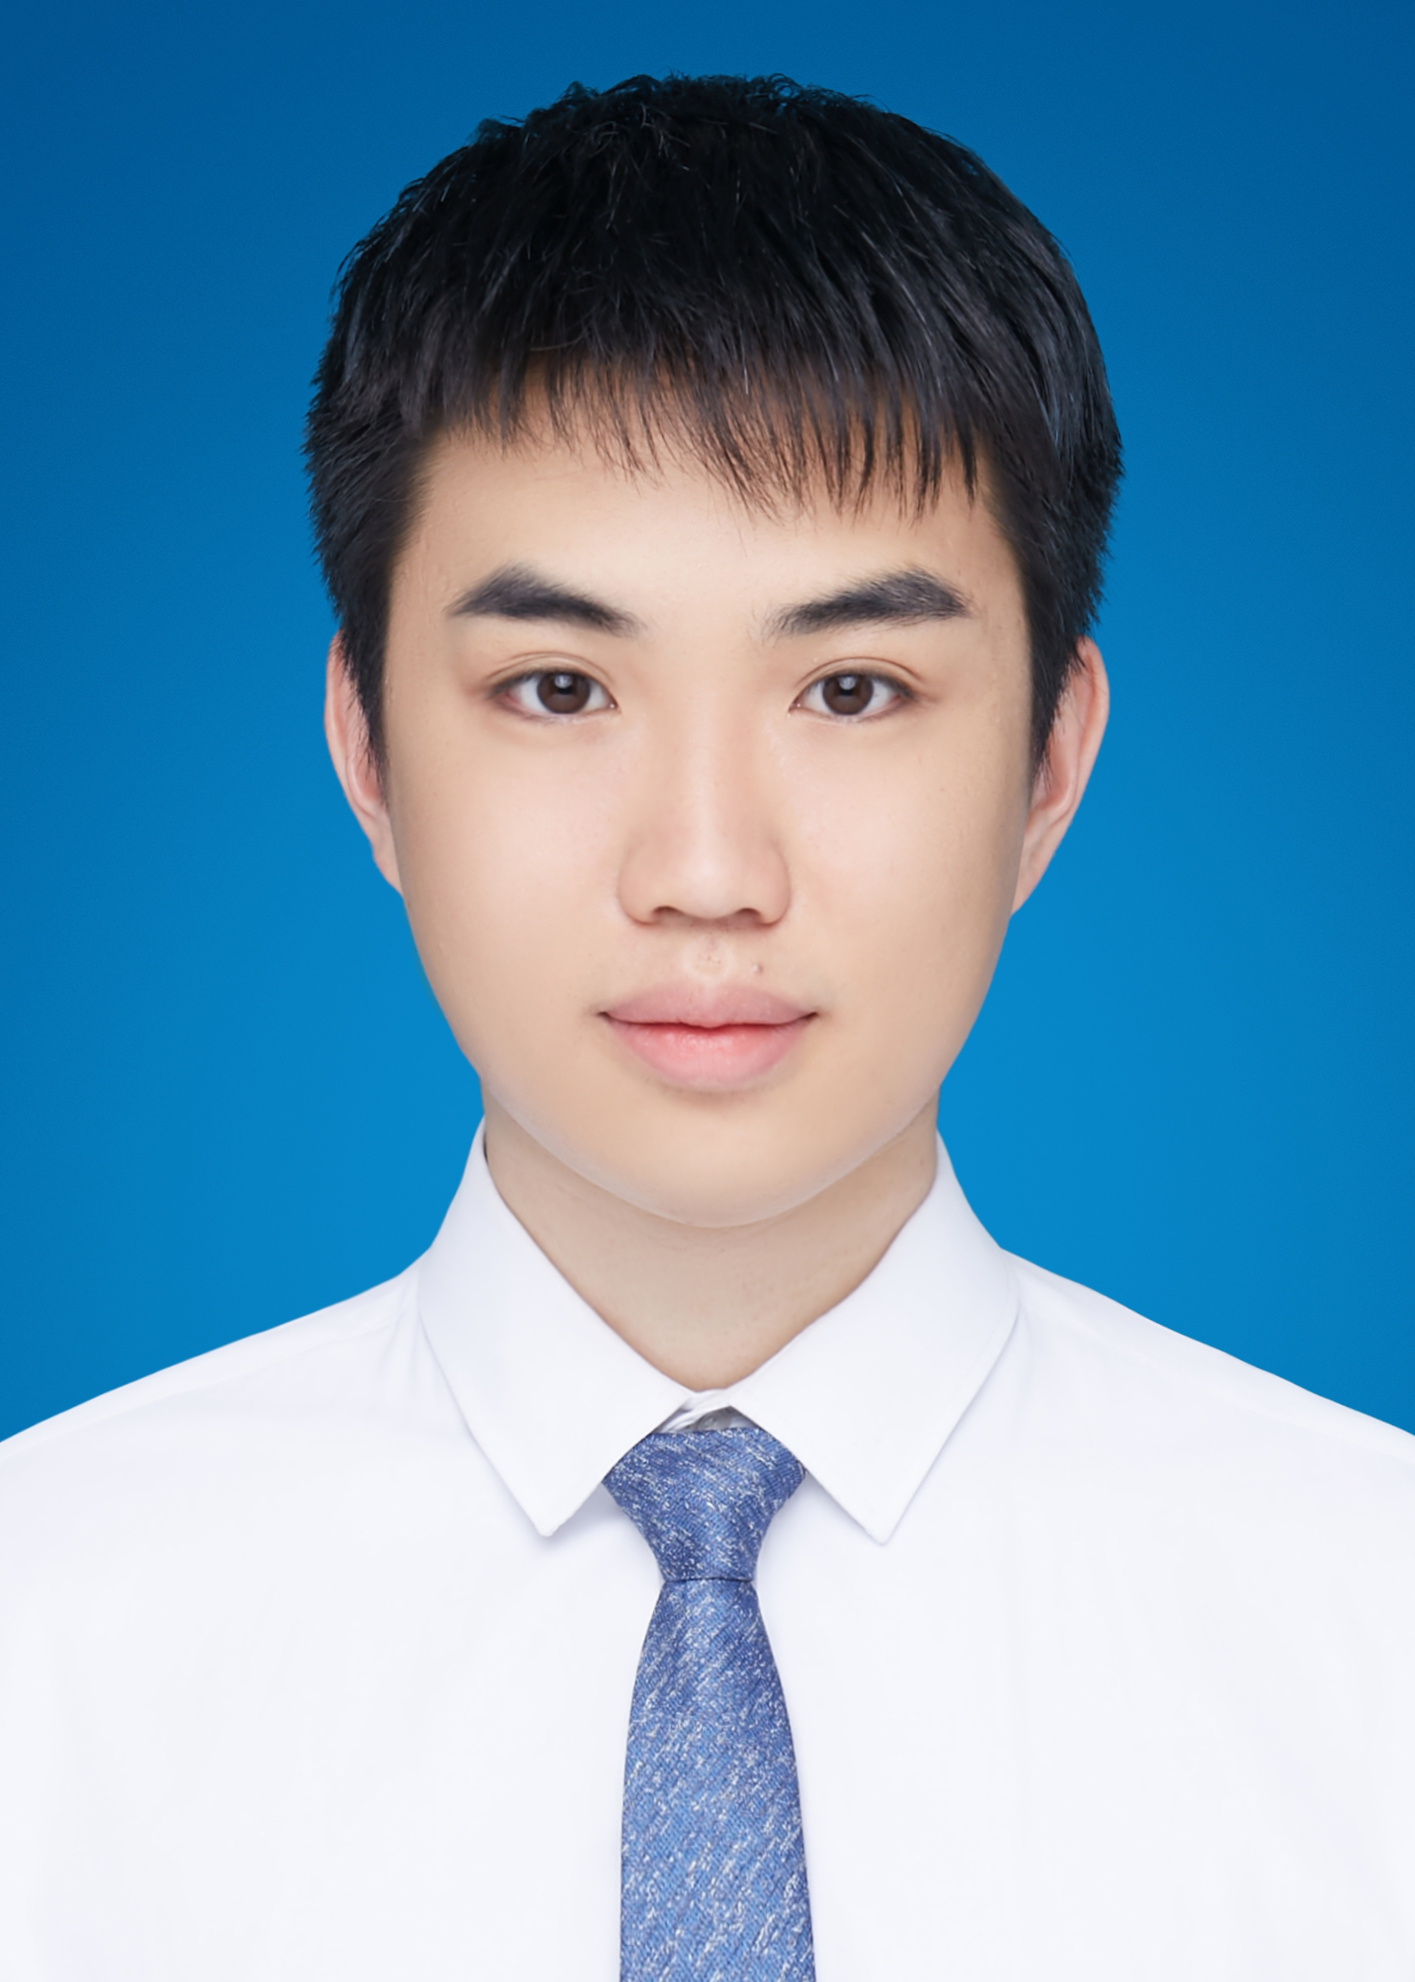
\includegraphics[width=2.2cm,clip]{person2.jpg}
}
\parbox{\dimexpr\linewidth-2.9cm\relax}{
\begin{tabularx}{\linewidth}{L L} \\
  \textbf{\Large \name} & {}\\
  % {Data of Birth: 17 December 1996} & {}
  % \\
  {\course} & {\href{\unisturl}{Department of Computer Science and Engineering, UNIST}}
  \\
  {Research: Quality Assurance for AI Infrastructure} & {E-mail: \href{mailto:\emaila}{\emaila}}
  \\
  {Homepage: \href{\homepage}{muyanzhou96.github.io}} & {Google Scholar: \href{\googlescholar}{Profile}}
  \\
  {ORCID: \href{\orcid}{0000-0003-1816-2246}} & {Research Areas: Software Testing, SE for AI, AI for SE}
  \\

  % Hometown Address: Room 305, Building 21, Southwest New Village, Jiangyin City & {}
\end{tabularx}
}


\vspace{-1.5mm}


%-----------EDUCATION-----------
\section{\textbf{Education and Experience}}
  \resumeSubHeadingListStart
    \resumeSubheading
      {UNIST}{\textbf{InnoCORE Project Postdoctoral Researcher } 2026.06-2026.11}
      {Department of Computer Science and Engineering}
      {\textbf{Supervisor}: Mijung Kim}

    \resumeSubheading
      {Nanjing University}{\textbf{Ph.D. in Software Engineering } 2022.09-2026.06}
      {Software College, Nanjing City
      }{\textbf{Supervisors}: Zhenyu Chen, Chunrong Fang \quad \textbf{Profession:} Software Engineering}
    
    \resumeSubheading
      {Tianjin University}{\textbf{Master's degree} 2019.09-2022.01}
      {College of Intelligence and Computing}
      {\textbf{Supervisors}: Zan Wang, Shuang Liu, Junjie Chen \quad \textbf{Profession}: Software Engineering}

    \resumeSubheading
      {Nantong University}{\textbf{Bachelor's degree} 2015.09-2019.06}
      {School of Computer Science and Technology
      }{\textbf{Supervisor}: Xiang Chen \quad \textbf{Profession}: Computer Science and Technology}
    
  \resumeSubHeadingListEnd
\vspace{-5.5mm}
%




\section{\textbf{Publications}}

    \subsection{\textbf{First-Author Publications}}
    \resumeItemListStart
    \item {\textbf{Yanzhou Mu}, Shuo Meng, Mijung Kim, Xiang Chen, Chunrong Fang, Zhenyu Chen, Juan Zhai. CIPIHunter: Detecting Configuration-Induced Prediction Instability in Deep Learning Frameworks. In Proceedings of IEEE/ACM Automated Software Engineering Conference (ASE 2026). ACM, Munich, Germany. CCF-A.}

\vspace{2mm}
    \item {\textbf{Yanzhou Mu}, Rong Wang, Juan Zhai, Chunrong Fang, Xiang Chen, Jiacong Wu, An Guo, Jiawei Shen, Bingzhuo Li, and Zhenyu Chen. Understanding LLM-Centric Challenges for Deep Learning Frameworks: An Empirical Analysis. ACM Transactions on Software Engineering and Methodology, 2026. CCF-A.}

    \vspace{2mm}
    \item {\textbf{Yanzhou Mu}, Rong Wang, Juan Zhai, Chunrong Fang, Xiang Chen, Peiran Yang, Zhixiang Cao, Ruixiang Qian, Shaoyu Yang, and Zhenyu Chen. Deep Learning Framework Testing via Model Mutation: How far are we? IEEE Transactions on Software Engineering, 2025. CCF-A.}

    \vspace{2mm}
    \item {\textbf{Yanzhou Mu}, Juan Zhai, Chunrong Fang, Xiang Chen, Zhixiang Cao, Peiran Yang, Kexin Zhao, An Guo and Zhenyu Chen. Improving Deep Learning Framework Testing with Model-Level Metamorphic Testing.
    International Symposium on Software Testing and Analysis (ISSTA 2025), Thondheim, Norway, 2025. CCF-A.}

    \vspace{2mm}
    \item {\textbf{Yanzhou Mu}, Juan Zhai, Chunrong Fang, Xiang Chen, Zhixiang Cao, Peiran Yang, Yinglong Zou, Tao Zheng, and Zhenyu Chen. DevMuT: Testing Deep Learning Framework via Developer Expertise-Based Mutation. In Proceedings of IEEE/ACM Automated Software Engineering Conference (ASE 2024). ACM, Sacramento, California, United States. CCF-A.}

    \vspace{2mm}
    \item {\textbf{Yanzhou Mu}, Zan Wang, Xiang Chen, Junjie Chen, Jingke Zhao, and Jianmin Wang. Deep learning test optimization method using multi-objective optimization. Chinese version: Journal of Software, 2022, 33(07):2499-2524, DOI:10.13328/j.cnki.jos.006583. English version: International Journal of Software \& Informatics, 12(4), 2022.}

    \vspace{2mm}
    \item {\textbf{Yanzhou Mu}, Zan Wang, Shuang Liu, Jun Sun, Junjie Chen, and Xiang Chen. HARS: Heuristic-enhanced adaptive randomized scheduling for concurrency testing. In 2021 IEEE 21st International Conference on Software Quality, Reliability and Security (QRS), pages 219-230. IEEE, 2021.}

    \vspace{2mm}
    \subsection{\textbf{Co-authored Publications}}
    \item {Yuan Xiao, Yuchen Chen, Jiaming Wang, Wei Song, Jun Sun, Shiqing Ma, \textbf{Yanzhou Mu}, Juan Zhai, Chunrong Fang, Jin Song Dong, and Zhenyu Chen. Train in Vain: Functionality-Preserving Poisoning to Prevent Unauthorized Use of Code Datasets. Findings of the Association for Computational Linguistics, 2026. CCF-A.}


    \vspace{2mm}
    \item {Yilong Zou, Juan Zhai, Chunrong Fang, \textbf{Yanzhou Mu}, Jiawei Liu and Zhenyu Chen. Deep Learning Framework Testing via Heuristic Guidance Based on Multiple Model Measurements, ACM Transactions on Software Engineering and Methodology, 2025, CCF-A}

    \vspace{2mm}
    \item {Xinxue Zhu, Jiacong Wu, Xiaoyu Zhang, Tianlin Li, \textbf{Yanzhou Mu}, Juan Zhai, Chao Shen, Chunrong Fang, and Yang Liu. An Empirical Study of Bugs in Modern LLM Agent Frameworks. The 2nd International Workshop on Large Language Model Supply Chain Analysis (LLMSC 2026), co-located with FSE 2026, 2026. \textbf{Accepted.}}
    
    \vspace{2mm}
    \item {An Guo, Shuoxiao Zhang, Enyi Tang, Xinyu Gao, Haomin Pang, Haoxiang Tian, \textbf{Yanzhou Mu}, Wu Wen, Chunrong Fang, and Zhenyu Chen. When Autonomous Vehicle Meets V2X Cooperative Perception: How Far Are We? The 40th IEEE/ACM International Conference on Automated Software Engineering, November 16-20, 2025, Seoul, South Korea. CCF-A.}

    \vspace{2mm}
    \item {Chunyu Zhao, \textbf{Yanzhou Mu}, Xiang Chen, Jingke Zhao, Xiaolin Ju, and Gan Wang. Can test input selection methods for deep neural network guarantee test diversity? A large-scale empirical study. Information and Software Technology, 150:106982, 2022. \textbf{Co-first Author.}}

    \vspace{2mm}
    \item {Xiang Chen, \textbf{Yanzhou Mu}, Ke Liu, Zhanqi Cui, and Chao Ni. Revisiting heterogeneous defect prediction methods: How far are we? Information and Software Technology, 130:106441, 2021. \textbf{Co-first Author.}}

    \vspace{2mm}
    \item {Xiang Chen, \textbf{Yanzhou Mu}, Yubin Qu, Chao Ni, Meng Liu, Tong He, and Shangqing Liu. Do different cross-project defect prediction methods identify the same defective modules? Journal of Software: Evolution and Process, 32(5):e2234, 2020. \textbf{Co-first Author.}}
    
    \subsection{\textbf{Earlier Publications}}
    \vspace{2mm}
    \item {Hao Li, Xiaohong Li, Xiang Chen, Xiaofei Xie, \textbf{Yanzhou Mu}, and Zhiyong Feng. Cross-project defect prediction via asttoken2vec and blstm-based neural network. In 2019 International Joint Conference on Neural Networks (IJCNN), pages 1-8. IEEE, 2019.}
    
    \vspace{2mm}
    \subsection{\textbf{Manuscripts and Preprints}}
    
    \item {Zhixiang Cao, Di Tian, Runwei Guan, \textbf{Yanzhou Mu}, Xiaolou Sun, Shaofeng Liang, Daizong Liu, Tao Huang, Yutao Yue, Henghui Ding, Bin Fang, Alex Zhou, Qing-Long Han, and Hui Xiong. Tactile-based Multimodal Fusion in Embodied Intelligence: A Survey of Vision, Language, and Contact-Driven Paradigms. arXiv preprint, under review, 2026. DOI:10.48550/arXiv.2605.17336. \textbf{Preprint.}}


    \vspace{2mm}
    \item {An Guo, Xinyu Gao, Chunrong Fang, Haoxiang Tian, Weisong Sun, \textbf{Yanzhou Mu}, Shuncheng Tang, Lei Ma, Xiapu Luo, and Zhenyu Chen. Generate Realistic Test Scenes for V2X Communication Systems.
    ACM Transactions on Software Engineering and Methodology, 2025, CCF-A, \textbf{Major revision.}}
     
    
    \resumeItemListEnd


%-----------Positions of Responsibility-----------------
\section{Project Experience}
\vspace{-0.4mm}
\resumeSubHeadingListStart




\resumePOR{MindSpore Model Generalization Testing Technology | (Completed, Student Leader)} % Position
    {} 
    {} % Tenure Period
\resumeItemListStart
\item {Developed a model structure generalization tool based on the domestic deep learning framework MindSpore. The tool extracts feature factors, ranges, and constraints of mainstream CV and NLP model architectures, modifies model structures, and performs testing to detect defects. \textbf{The project results were an essential part in supporting the collaboration team to win the Huawei 2023 Innovation Testing Application Award.}}
\resumeItemListEnd
    
\resumePOR{Research on Key Mutation Testing Techniques for DL Frameworks | (Ongoing, Student Leader)} % Position
    {} 
    {} % Tenure Period
    \resumeItemListStart
	    \item {Designed mutation rules that simulate actual user development operations to generate test models aligned with practical scenarios. Evaluated the diversity and sufficiency of test data by integrating static and dynamic framework features. Employed heuristic methods to guide mutation testing and combined experience replay to improve testing efficiency and quality. \textbf{Project results were published at ASE 2024, and a patent application for an invention is underway.}}
\resumeItemListEnd

\resumePOR{Fast Detection, Localization, and Patch Generation for Concurrency Defects | (Completed, Project Participant)} % Position
    {} % Club, Event
    {} % Tenure Period
    \vspace{-2.0mm}
    \resumeItemListStart
    \item {Designed a heuristic scheduling testing method to optimize Java concurrent programs, enhancing detection efficiency and effectiveness. \textbf{Project results were published at the CCF-C conference QRS'21 and granted an invention patent.}}

   
    \resumeItemListEnd

	    \resumePOR{Generalization Testing for Large-Model Frameworks | (Completed, Student Leader)} % Position
    {} 
    {} % Tenure Period
    \resumeItemListStart
    \item {Developed a generalization testing framework for large-model training systems by decomposing models into reusable structural modules and generating semantically meaningful variants across model structure, parallelism, and optimization. Investigated configuration constraints spanning model, parallelism, optimization, and backend layers, distinguishing semantic requirements from implementation restrictions while preserving mutation intent during deep distributed execution. Applied cross-framework differential testing across PTA and MindSpore-based stacks. \textbf{Produced 52 issue reports, including 44 high-confidence suspected framework defects.}}
\resumeItemListEnd

    
\resumeSubHeadingListEnd
\vspace{-5mm}
  % \resumeSubHeadingListStart
  %   \resumeSubheading
  %     { Can test input selection methods for deep neural network guarantee test diversity? a large-scale empirical study. Information and Software Technology, 150:106982, 2022.}{City}
  %     {Your Role}{Event dates}
     
    
  %   \vspace{-3.0mm}
    
  %   \resumeSubheading
  %     {Company Name}{City}
  %     {Your Role}{Event dates}
      
  %   \vspace{-3.0mm}
    
  %   \resumeSubheading
  %     {Company Name}{City}
  %     {Your Role}{Event dates}
      
      
  % \resumeSubHeadingListEnd
% \vspace{-8.5mm}



% %-----------PROJECTS-----------------
% \section{\textbf{Travel Plan}}
% \resumeSubHeadingListStart

%     \resumeProject
%       {Project Name} %Project Name
%       {Project description(Your input in the project)} %Project Name, Location Name
%       {Event dates} %Event Dates

%       \resumeItemListStart
%         \item {Tools \& technologies used: xxx,xxx}
%         \item {More description on the project(The output you achieved by working on the project)}
%     \resumeItemListEnd
%     \vspace{-2mm}
    
%     \resumeProject
%       {Project Name} %Project Name
%       {Project description(Your input in the project)} %Project Name, Location Name
%       {Event dates} %Event Dates

%       \resumeItemListStart
%         \item {Tools \& technologies used: xxx,xxx}
%         \item {More description on the project(The output you achieved by working on the project)}
%     \resumeItemListEnd
%     \vspace{-2mm}
    
      
%   \resumeSubHeadingListEnd
% \vspace{-5.5mm}









% %-----------Technical skills-----------------
% \section{\textbf{Technical Skills and Interests}}
%  \begin{itemize}[leftmargin=0.1in, label={}]
%     \small{\item{
%      \textbf{Languages: }{Chinese and English.} \\
%      \textbf{Interests: }{Swim, Guitar, Go, and Badminton.} \\
%      \textbf{Technical Skills: }{Microsoft Office, Matlab, R, C++, Java, and Python.} \\
%     }}
%  \end{itemize}
%  \vspace{-16pt}







\section{\textbf{Patent}}

    \resumeItemListStart

    \item {\textbf{Yanzhou Mu}; Zan Wang; Shuang Liu. A heuristic rule-based concurrent adaptive random testing method. Patent No: CN113468047A.}

    \item {Junjie Chen; \textbf{Yanzhou Mu}; Zan Wang; Jianmin Wang; Jiao Jia. A multi-objective optimization-based method for selecting deep learning test inputs. Patent No: CN114721934A.}
    
    \item {Zhenyu Chen; Yidong Ke; Jiawei Liu; \textbf{Yanzhou Mu}. A neural network fuzz testing method guided by mutation image entropy values. Patent No: CN117218051A.}
    
    \item {Yongping Liu; Zhenyu Chen; Chunrong Fang; \textbf{Yanzhou Mu}; Ruifa Luo; Shuiyong Du. Mutation testing method, device, and computer equipment based on neuron characteristics of intelligent traffic models. Patent No: CN118689772A.}
    
    \item {Yongping Liu; Zhenyu Chen; Chunrong Fang; \textbf{Yanzhou Mu}; Ruifa Luo; Shuiyong Du. Domain-specific mutation testing method, device, and computer equipment based on intelligent traffic V2X models. Patent No: CN118689771A.}
    
    \item {Zhijin Guan; Haiying Ma; Hehe Gu; Zongyuan Zhang; \textbf{Yanzhou Mu}; Jing Zhao; Meng Liu. A quantum circuit image recognition method. Patent No: CN106997462A.}

    
    % \item {程实; 施佺; \textbf{沐燕舟}; 何金凤.具有除尘功能的计算机机箱.专利号：CN110825176A.} 
    
    % \item {程实; 宋驰; 李春桥; \textbf{沐燕舟}; 何金凤.一种自平衡稳定式虚拟现实眼镜.专利号：C207571395U.} 

    
    \resumeItemListEnd

%-----------Achievements-----------------
\section{\textbf{Awards and Honors}}
\vspace{-0.4mm}
\resumeSubHeadingListStart
\resumePOR{Nanjing University-Jiangsu Bank Scholarship} % Award
    {} % Event
    {2024.10} %Event Year

\resumePOR{Huawei 2023 Innovation Testing Application Award} % Award
    {} % Event
    {2023.11} %Event Year

\resumePOR{Outstanding Graduate of Tianjin University} % Award
    {} % Event
    {2022.06} %Event Year

\resumePOR{Outstanding Communist Youth League Member of Tianjin University} % Award
    {} % Event
    {2021.01} %Event Year

\resumePOR{Outstanding Undergraduate Graduation Project/Thesis of Nantong University, Class of 2019} % Award
    {} % Event
    {2019.06} %Event Year

\resumePOR{Outstanding Student Cadre of Jiangsu Province} % Award
    {} % Event
    {2018.05} %Event Year

\resumePOR{National Scholarship for Undergraduate Students} % Award
    {} % Event
    {2017.11} %Event Year

\resumePOR{Merit Student of Nantong City} % Award
    {} % Event
    {2017.05} %Event Year

\resumePOR{Model Merit Student of Nantong University} % Award
    {} % Event
    {2016.09} %Event Year


\resumeSubHeadingListEnd
\vspace{-5mm}


% \section{\textbf{其它经历}}

%     \resumeItemListStart
%     \item {南京大学新生学院党建辅导员}
%     \item {南京大学新生学院开甲书院党支部宣传委员}
%     \item {天津大学智能与计算学部2019级软件工程第六党支部副书记}
%  \resumeItemListEnd
 
\end{document}
